% Template adapted from https://github.com/jgm/pandoc-templates/blob/master/default.latex
% To be used with XeLaTex in memoiR
%%%%%%%%%%%%%%%%%%%%%%%%%%%%%%%%%%%%%%%%%%%%%%%%%%%%%%%%%%%%%%%%%%%%%%%%%%%%%%%%%%%%%%%%%

% Options for packages loaded elsewhere
\PassOptionsToPackage{unicode=true}{hyperref}
\PassOptionsToPackage{hyphens}{url}
\PassOptionsToPackage{dvipsnames,svgnames*,x11names*}{xcolor}
% Right to left support


\documentclass[
  10pt,
  italian,
  a4paper,
  extrafontsizes,onecolumn,openright
  ]{memoir}

% Double (or whatever) spacing

% Math
\usepackage{amssymb, amsmath}
% mathspec: arbitrary math fonts
\usepackage{unicode-math}
\defaultfontfeatures{Scale=MatchLowercase}
\defaultfontfeatures[\rmfamily]{Ligatures=TeX,Scale=1}

% Fonts
\usepackage{lmodern}
\usepackage{fontspec}

% Main font
% Specific sanserif font
% Specific monotype font
\setmonofont[Scale=0.75]{Operator Mono SSm Lig Book}
% Specific math font
% Chinese, Japanese, Corean fonts

% Use upquote for straight quotes in verbatim environments
\usepackage{upquote}
% Use microtype
\usepackage[]{microtype}
\UseMicrotypeSet[protrusion]{basicmath} % disable protrusion for tt fonts

% Verbatim in note

% Color links
\usepackage{xcolor}

% Strikeout

% Necessary for code chunks

% Listings package

% Tables
\usepackage{longtable,booktabs,tabu}
% Fix footnotes in tables (requires footnote package)
\IfFileExists{footnote.sty}{\usepackage{footnote}\makesavenoteenv{longtable}}{}

% Graphics
\usepackage{graphicx,grffile}
\graphicspath{{images/}}
\makeatletter
\def\maxwidth{\ifdim\Gin@nat@width>\linewidth\linewidth\else\Gin@nat@width\fi}
\def\maxheight{\ifdim\Gin@nat@height>\textheight\textheight\else\Gin@nat@height\fi}
\makeatother
% Scale images if necessary, so that they will not overflow the page
% margins by default, and it is still possible to overwrite the defaults
% using explicit options in \includegraphics[width, height, ...]{}
\setkeys{Gin}{width=\maxwidth,height=\maxheight,keepaspectratio}

% Prevent overfull lines
\setlength{\emergencystretch}{3em}  
\providecommand{\tightlist}{%
  \setlength{\itemsep}{0pt}\setlength{\parskip}{0pt}}

% Number sections for memoir (secnumdepth counter is ignored)
\setsecnumdepth{section}

% Set default figure placement to htbp
\makeatletter
\def\fps@figure{htbp}
\makeatother

% Spacing in lists
\usepackage{enumitem}

% Polyglossia
\usepackage{polyglossia}
\setmainlanguage{it}
\setotherlanguage{en-US}

% BibLaTeX
\usepackage[backend=biber,style=authoryear-ibid,isbn=false,backref=true,giveninits=true,uniquename=init,maxcitenames=2,maxbibnames=150,sorting=nyt,sortcites=false,style=apa]{biblatex}
\addbibresource{refs.bib}

% cslreferences environment required by pandoc > 2.7



%%%%%%%%%%%%%%%%%%%%%%%%%%%%%%%%%%%%%%%%%%%%%%%%%%%%%%%%%%
% memoiR format

% Chapter Summary environment 
\usepackage[tikz]{bclogo}
\newenvironment{Summary}
  {\begin{bclogo}[logo=\bctrombone, noborder=true, couleur=lightgray!50]{In breve}\parindent0pt}
  {\end{bclogo}}
% Syntax:
%
%```{block, type='Summary'}
% Deliver message here.
% ```

% scriptsize code 
\let\oldverbatim\verbatim
\def\verbatim{\oldverbatim\scriptsize}
% Applies to code blocks and R code results
% code chunk options size='scriptsize' applies only to R code and results
% if the code chunk sets a different size, \def\verbatim{...} is prioritary for code results 


% Layout
%%%%%%%%%%%%%%%%%%%%%%%%%%%%%%%%%%%%%%%%%%%%%%%%%%%%%%%%%%

% Based on memoir, style companion
\newcommand{\MemoirChapStyle}{daleif1}
\newcommand{\MemoirPageStyle}{Ruled}

% Space between paragraphs
\usepackage{parskip}
  \abnormalparskip{3pt}

% Adjust margin paragraphs vertical position
\usepackage{marginfix}


% Margins
%%%%%%%%%%%%%%%%%%%%%%%%%%%%%%%%%%%%%%%

% allow use of '-',+','/' ans '*' to make simple length computation
\usepackage{calc}

% Full-width figures utilities
\newlength\widthw % full width
\newlength{\rf}
\newcommand*{\definesHSpace}{
  \strictpagecheck % slower but efficient detection of odd/even pages
  \checkoddpage
  \ifoddpage
  \setlength{\rf}{0mm}
  \else
  \setlength{\rf}{\marginparsep+\marginparwidth}
  \fi
}

\makeatletter
% 1" margins for the front matter.
\newcommand*{\SmallMargins}{
  \setlrmarginsandblock{1.5in}{1.5in}{*}
  \setmarginnotes{0.1in}{0.1in}{0.1in}
 \setulmarginsandblock{1.5in}{1in}{*}
  \checkandfixthelayout
  \ch@ngetext
  \clearpage
  \setlength{\widthw}{\textwidth+\marginparsep+\marginparwidth}
  \footnotesatfoot
  \chapterstyle{\MemoirChapStyle}  % Chapter and page styles must be recalled
  \pagestyle{\MemoirPageStyle}
}

% 3" outer margin for the main matter
\newcommand{\LargeMargins}{\SmallMargins}
\makeatother

% Figure captions and footnotes in outer margins


% Main title page with filigrane
%%%%%%%%%%%%%%%%%%%%%%%%%%%%%%%%%%%%%%%%%%%%%%%%%%%%%%%%%%

% Text blocks
\usepackage[absolute,overlay]{textpos}
  \setlength{\TPHorizModule}{1mm}
  \setlength{\TPVertModule}{1mm}

\newcommand{\MainTitlePage}[2]{
  \SmallMargins % Margins
  \pagestyle{empty} % No header/footer
  \textblockorigin{\stockwidth-\paperwidth-\trimedge}{\trimtop} % recto
  \begin{textblock*}{2mm}(\spinemargin/2,\uppermargin/2)
    \rule{1pt}{\paperheight-\uppermargin}
  \end{textblock*}
  \begin{textblock*}{\paperwidth*2/3}(\paperwidth/5, \paperheight/5)
    \flushright
    \begin{Spacing}{3}
      {\fontfamily{qtm}\selectfont\fontsize{45}{45}\selectfont\textsc{\thetitle}}
    \end{Spacing}
  \end{textblock*}
    \begin{textblock*}{\paperwidth*2/3}(\paperwidth/5, \paperheight/2)
    \flushright
    {\fontfamily{qtm}\huge\theauthor}
  \end{textblock*}
    \begin{textblock*}{\paperwidth*2/3}[0, 1](\spinemargin, \uppermargin+\textheight)
    \normalfont\thedate
  \end{textblock*}
  ~\\ % Print a character or the page will not exist
  \newpage
  \textblockorigin{\trimedge}{\trimtop} % verso
  \begin{textblock*}{\textwidth}(\paperwidth-\spinemargin-\textwidth, \uppermargin)
    #1
  \end{textblock*}
  \begin{textblock*}{\textwidth}[0,1](\paperwidth-\spinemargin-\textwidth, \uppermargin+\textheight+\footskip)
    \centering
    
\includegraphics[width=\paperwidth/4]{logo}\\ \bigskip
    #2
  \end{textblock*}
  ~\\ % Print a character or the page will not exist
  \newpage
}

% Clear page and open an even one (\clearpage opens an odd one)
\newcommand{\evenpage}{
  \clearpage
  \strictpagecheck % slower but efficient detection of odd/even pages
  \checkoddpage
  \ifoddpage
    \thispagestyle{empty}
    ~\\ % Print a character or the page will not exist
    \newpage
  \else
    % do nothing
  \fi
}


%% PDF title page to insert
%%%%%%%%%%%%%%%%%%%%%%%%%%%%%%%%%%%%%%%%%%%%%%%%%%%%%%%%%%



%% Bibliography
%%%%%%%%%%%%%%%%%%%%%%%%%%%%%%%%%%%%%%%%%%%%%%%%%%%%%%%%%%

\usepackage[strict,autostyle]{csquotes}
% Repeated citation as author-year-title instead of author-title (modification of footcite:note in verbose-inote.cbx)

%% Table of Contents
%%%%%%%%%%%%%%%%%%%%%%%%%%%%%%%%%%%%%%%%%%%%%%%%%%%%%%%%%%

% fix the typesetting of the part number
\renewcommand\partnumberlinebox[2]{#2\ ---\ }


% Fonts
%%%%%%%%%%%%%%%%%%%%%%%%%%%%%%%%%%%%%%%%%%%%%%%%%%%%%%%%%%


% Hyperref comes last
%%%%%%%%%%%%%%%%%%%%%%%%%%%%%%%%%%%%%%%%%%%%%%%%%%%%%%%%%%

\usepackage{hyperref}
\hypersetup{
  pdftitle={Psicometria},
  pdfauthor={Corrado Caudek},
  colorlinks=true,
  linkcolor=Maroon,
  citecolor=Blue,
  urlcolor=Blue,
  breaklinks=true}

% Don't use monospace font for urls
\urlstyle{same}


% Title, author, date from YAML to LaTeX
%%%%%%%%%%%%%%%%%%%%%%%%%%%%%%%%%%%%%%%%%%%%%%%%%%%%%%%%%%

\title{Psicometria}

\author{Corrado Caudek}

\date{2021-12-21}


% Include headers (preamble.tex) here
%%%%%%%%%%%%%%%%%%%%%%%%%%%%%%%%%%%%%%%%%%%%%%%%%%%%%%%%%%
% Add LaTeX code into the preamble of the document here
\hyphenation{bio-di-ver-si-ty sap-lings}


%%%%%%%%%%%%%%%%%%%%%%%%%%%%%%%%%%%%%%%%%%%%%%%%%%%%%%%%%%%%%%%%%%%%%%%%%
% memoiR dalef3 chapter style 
% https://ctan.crest.fr/tex-archive/info/latex-samples/MemoirChapStyles/MemoirChapStyles.pdf
\usepackage{soul}
\definecolor{nicered}{rgb}{.647,.129,.149}

\makeatletter
\makechapterstyle{pedersen}
\makeatother



%\makeatletter
%\newlength\dlf@normtxtw
%\setlength\dlf@normtxtw{\textwidth}
%\def\myhelvetfont{\def\sfdefault{mdput}}
%\newsavebox{\feline@chapter}
%\newcommand\feline@chapter@marker[1][4cm]{%
%  \sbox\feline@chapter{%
%    \resizebox{!}{#1}{\fboxsep=1pt%
%	  \colorbox{nicered}{\color{white}\bfseries\sffamily\thechapter}%
%	}}%
%  \rotatebox{90}{%
%    \resizebox{%
%	  \heightof{\usebox{\feline@chapter}}+\depthof{\usebox{\feline@chapter}}}%
%	{!}{\scshape\so\@chapapp}}\quad%
%  \raisebox{\depthof{\usebox{\feline@chapter}}}{\usebox{\feline@chapter}}%
% }
%\newcommand\feline@chm[1][4cm]{%
%  \sbox\feline@chapter{\feline@chapter@marker[#1]}%
%  \makebox[0pt][l]{% aka \rlap
%    \makebox[1cm][r]{\usebox\feline@chapter}%
%  }}
%\makechapterstyle{pedersen}{ %daleif1
%
%  \renewcommand\chapnamefont{\normalfont\Large\scshape\raggedleft\so}
%  
%  % I changed this!!
%  %\renewcommand\chaptitlefont{\normalfont\huge\bfseries\scshape\color{nicered}}
%  \renewcommand\chaptitlefont{\normalfont\huge\fontencoding{T1}\fontfamily{phv}\selectfont\color{nicered}}
%    
%  \renewcommand\chapternamenum{}
%  \renewcommand\printchaptername{}
%  \renewcommand\printchapternum{\null\hfill\feline@chm[2.5cm]\par}
%  \renewcommand\afterchapternum{\par\vskip\midchapskip}
%  \renewcommand\printchaptertitle[1]{\chaptitlefont\raggedleft ##1\par}
%}
%\makeatother

\DeclareMathOperator{\Var}{Var} % Define variance operator
\DeclareMathOperator{\SD}{SD} % Define sd operator
\DeclareMathOperator{\Cov}{Cov} % Define covariance operator
\DeclareMathOperator{\Corr}{Corr} % Define correlation operator
\DeclareMathOperator{\Me}{Me} % Define mediane operator
\DeclareMathOperator{\Mo}{Mo} % Define mode operator
\DeclareMathOperator{\Bin}{Bin} % Define binomial operator
\DeclareMathOperator{\Bernoulli}{Bernoulli} % Define Bernoulli operator
\DeclareMathOperator{\Poi}{Poi} % Define Poisson operator
\DeclareMathOperator{\Uniform}{Uniform} % Define Uniform operator
\DeclareMathOperator{\Cauchy}{Cauchy} % Define Cauchy operator
\DeclareMathOperator{\elpd}{elpd} % Define elpd operator
\DeclareMathOperator{\lppd}{lppd} % Define lppd operator
\DeclareMathOperator{\LOO}{LOO} % Define LOO operator
\DeclareMathOperator{\B}{\mathscr{B}} % Define Bernoulli operator
\newcommand{\R}{\textsf{R}} % Define R programming language symbol
\newcommand{\E}{\mathbb{E}} % Define expected value operator
\newcommand{\Real}{\mathbb{R}} % Define real number operator
\newcommand{\Prob}{\mathscr{P}}
\DeclareMathOperator*{\argmin}{arg\,min} % thin space, limits on side in displays
\DeclareMathOperator*{\argmax}{arg\,max} % thin space, limits on side in displays

\raggedbottom % allow variable (ragged) site heights
\frenchspacing

\usepackage[
  labelfont=bf, 
  font={small, it} 
]{caption} 
\usepackage{upquote} % print correct quotes in verbatim-environments
\usepackage{empheq} 
\usepackage{xfrac}
\usepackage{lstbayes}


% Introduction to Modern statistics ------------------------------------------------
% https://github.com/OpenIntroStat/ims/blob/main/latex/ims-style.tex

\usepackage[framemethod=tikz]{mdframed} 
\usepackage{helvet} 
\usepackage{xcolor}


\definecolor{oiB}{HTML}{000000}            % COL["blue","full"]
\definecolor{oiLB}{HTML}{e0e0e0}           % lighter version of oiB

\definecolor{oiY}{HTML}{000000}            % COL["yellow","full"]
\definecolor{oiLY}{HTML}{e0e0e0}           % lighter version of oiY

\definecolor{oiR}{HTML}{000000}            % COL["red","full"]
\definecolor{oiLR}{HTML}{e0e0e0}           % lighter version of oiR

\definecolor{oiGray}{HTML}{808080}         % COL["gray","full"]
\definecolor{oiLGray}{HTML}{f8f8f8}        % lighter version of oiR

\definecolor{oiGB}{rgb}{0.5,0.5,.5}        % from OS4 - for footnotes


% Helper environments ------------------------------------------------------------

% mdframedwithfootChapterintro: for chapterintro box

\newenvironment{mdframedwithfootChapterintro}
{   
    \savenotes
    \begin{mdframed}[%
    topline=true, bottomline=true, linecolor=oiB, linewidth=1.4pt,
    rightline=false, leftline=false,
    backgroundcolor=oiLB]
    %\stepcounter{footnote} % don't increment footnote counter
    \renewcommand{\thempfootnote}{\arabic{footnote}}
    }
{
    \end{mdframed}
    \spewnotes
}


% mdframedwithfootGPWE: for guidedpractice and workedexample

\newenvironment{mdframedwithfootGPWE}
{   
    \savenotes
    \begin{mdframed}[%
    topline=true, bottomline=true, linecolor=oiB, linewidth=0.5pt,
    rightline=false, leftline=false,
    backgroundcolor=oiLGray]
    %\stepcounter{footnote}
    \renewcommand{\thempfootnote}{\arabic{footnote}}
    }
{
    \end{mdframed}
    \spewnotes
}


% mdframedwithfootImportant: for important

\newenvironment{mdframedwithfootImportant}
{   
    \savenotes
    \begin{mdframed}[%
    topline=true, bottomline=true, linecolor=oiR, linewidth=0.5pt,
    rightline=false, leftline=false,
    backgroundcolor=oiLGray]
    %\stepcounter{footnote}
    \renewcommand{\thempfootnote}{\arabic{footnote}}
    }
{
    \end{mdframed}
    \spewnotes
}


% mdframedwithfootTip: for tip, data, and pronunciation

\newenvironment{mdframedwithfootTipDataPro}
{   
    \savenotes
    \begin{mdframed}[%
    topline=true, bottomline=true, linecolor=oiGray, linewidth=0.5pt,
    rightline=false, leftline=false,
    backgroundcolor=oiLGray]
    %\stepcounter{footnote}
    \renewcommand{\thempfootnote}{\arabic{footnote}}
    }
{
    \end{mdframed}
    \spewnotes
}


% Custom environments/boxes -------------------------------------------------------

% chapterintro

\newenvironment{chapterintro}{
\vspace{4mm}
\begin{mdframedwithfootChapterintro}
\begin{minipage}[t]{0.10\textwidth}
{$\:$ \\ \setkeys{Gin}{width=2.5em,keepaspectratio}
\includegraphics{images/_icons/chapterintro.png}}
\end{minipage}
\hfill
\begin{minipage}[t]{0.90\textwidth}
\setlength{\parskip}{1em}
\large
}{\end{minipage}
\end{mdframedwithfootChapterintro}
\vspace{4mm}
}

% guidedpractice

\newenvironment{guidedpractice}{
\vspace{4mm}
\begin{mdframedwithfootGPWE}
\begin{minipage}[t]{0.10\textwidth}
{$\:$ \\ \setkeys{Gin}{width=2.5em,keepaspectratio}
\includegraphics{images/_icons/guided-practice.png}}
\end{minipage}
\hfill
\begin{minipage}[t]{0.90\textwidth}
\vspace{-2mm}
\setlength{\parskip}{1em}
\noindent\textbf{\color{oiB}\small\fontencoding{T1}\fontfamily{phv}\selectfont{\MakeUppercase{Pratica guidata}}} $\:$ \\ \\
}{\end{minipage}
\end{mdframedwithfootGPWE}
\vspace{4mm}
}


% workedexample

\newenvironment{workedexample}{
    \let\oldrule\rule
    \renewcommand{\rule}[2]{\vspace{-2mm}\oldrule{##1}{##2}\vspace{-2mm}}
\vspace{4mm}
\begin{mdframedwithfootGPWE}
\begin{minipage}[t]{0.10\textwidth}
{$\:$ \\ \setkeys{Gin}{width=2.5em,keepaspectratio}
\includegraphics{images/_icons/worked-example.png}}
\end{minipage}
\hfill
\begin{minipage}[t]{0.90\textwidth}
\vspace{-2mm}
\setlength{\parskip}{1em}
\noindent\textbf{\color{oiB}\small\fontencoding{T1}\fontfamily{phv}\selectfont{\MakeUppercase{Esempio}}} $\:$ \\ \\
}{\end{minipage}
\end{mdframedwithfootGPWE}
\vspace{4mm}
}


% important

\newenvironment{important}{
    \let\oldtextbf\textbf
    \renewcommand{\textbf}[1]{{\textcolor{oiR}{\oldtextbf{##1}}}}
\vspace{4mm}
\begin{mdframedwithfootImportant}
\begin{minipage}[t]{0.10\textwidth}
{$\:$ \\ \setkeys{Gin}{width=2.5em,keepaspectratio}
\includegraphics{images/_icons/important.png}}
\end{minipage}
\hfill
\begin{minipage}[t]{0.90\textwidth}
\vspace{-2mm}
\setlength{\parskip}{1em}
}{\end{minipage}
\end{mdframedwithfootImportant}
\vspace{4mm}
}

% tip

\newenvironment{tip}{
\vspace{4mm}
\begin{mdframedwithfootTipDataPro}
\begin{minipage}[t]{0.10\textwidth}
{$\:$ \\ \setkeys{Gin}{width=2em,keepaspectratio}
\includegraphics{images/_icons/tip.png}}
\end{minipage}
\hfill
\begin{minipage}[t]{0.90\textwidth}
\vspace{-2mm}
\setlength{\parskip}{1em}
}{\end{minipage}
\end{mdframedwithfootTipDataPro}
\vspace{4mm}
}

% data

\newenvironment{data}{
\vspace{4mm}
\begin{mdframedwithfootTipDataPro}
\begin{minipage}[t]{0.10\textwidth}
{$\:$ \\ \setkeys{Gin}{width=2em,keepaspectratio}
\includegraphics{images/_icons/data.png}}
\end{minipage}
\hfill
\begin{minipage}[t]{0.90\textwidth}
\vspace{-2mm}
\setlength{\parskip}{1em}
}{\end{minipage}
\end{mdframedwithfootTipDataPro}
\vspace{4mm}
}

%\usepackage{titlesec}
%\titleformat{\chapter}[display]
%  {\normalfont\sffamily\huge\bfseries\color{blue}}
%  {\chaptertitlename\ \thechapter}{20pt}{\Huge}
%\titleformat{\section}
%  {\normalfont\sffamily\Large\bfseries\color{cyan}}
%  {\thesection}{1em}{}

%%%%%%%%%%%%%%%%%%%%%%%%%%%%


\usepackage{booktabs}
\usepackage{longtable}
\usepackage{array}
\usepackage{multirow}
\usepackage{wrapfig}
\usepackage{float}
\usepackage{colortbl}
\usepackage{pdflscape}
\usepackage{tabu}
\usepackage{threeparttable}
\usepackage{threeparttablex}
\usepackage[normalem]{ulem}
\usepackage{makecell}
\usepackage{xcolor}


% End of preamble
%%%%%%%%%%%%%%%%%%%%%%%%%%%%%%%%%%%%%%%%%%%%%%%%%%%%%%%%%%


\usepackage{amsthm}
\newtheorem{theorem}{Teorema}[chapter]
\newtheorem{lemma}{Lemma}[chapter]
\newtheorem{corollary}{Corollario}[chapter]
\newtheorem{proposition}{Proposizione}[chapter]
\newtheorem{conjecture}{Congettura}[chapter]
\theoremstyle{definition}
\newtheorem{definition}{Definizione}[chapter]
\theoremstyle{definition}
\newtheorem{example}{Esempio}[chapter]
\theoremstyle{definition}
\newtheorem{exercise}{Esercizio}[chapter]
\theoremstyle{definition}
\newtheorem{hypothesis}{Hypothesis}[chapter]
\theoremstyle{remark}
\newtheorem*{remark}{Osservazione}
\newtheorem*{solution}{Soluzione}
\begin{document}
\frontmatter

% Title page
%%%%%%%%%%%%%%%%%%%%%%%%%%%%%%%%%%%%%%%%%%%%%%%%%%%%%%%%%%


\MainTitlePage{Questo documento è stato realizzato con:

\begin{itemize}
  \item \LaTeX\; e la classe memoir (\url{http://www.ctan.org/pkg/memoir});
  \item $\R$ (\url{http://www.r-project.org/}) e RStudio (\url{http://www.rstudio.com/});
  \item bookdown (\url{http://bookdown.org/}) e memoiR (\url{https://ericmarcon.github.io/memoiR/}).
\end{itemize}}{Nel blog della mia pagina personale sono forniti alcuni approfondimenti degli argomenti qui trattati.

\url{https://ccaudek.github.io/caudeklab/}}


% Before Body
%%%%%%%%%%%%%%%%%%%%%%%%%%%%%%%%%%%%%%%%%%%%%%%%%%%%%%%%%%





% Contents
%%%%%%%%%%%%%%%%%%%%%%%%%%%%%%%%%%%%%%%%%%%%%%%%%%%%%%%%%%

\LargeMargins
{
\hypersetup{linkcolor=}
\setcounter{tocdepth}{2}
\tableofcontents
}


% Body
%%%%%%%%%%%%%%%%%%%%%%%%%%%%%%%%%%%%%%%%%%%%%%%%%%%%%%%%%%

\LargeMargins
\scriptsize

\normalsize

\chapter*{}

\vfill

\scriptsize

\normalsize

\scriptsize

Copyright \(\copyright\) 2022.

\normalsize

Data della versione presente: Dicembre 21, 2021.

\hypertarget{prefazione}{%
\chapter{Prefazione}\label{prefazione}}

\textbf{Data Science per psicologi} contiene il materiale delle lezioni dell'insegnamento di \emph{Psicometria B000286} (A.A. 2021/2022) rivolto agli studenti del primo anno del Corso di Laurea in Scienze e Tecniche Psicologiche dell'Università degli Studi di Firenze.

L'insegnamento di Psicometria si propone di fornire agli studenti un'introduzione all'analisi dei dati in psicologia.
Le conoscenze/competenze che verranno sviluppate in questo insegnamento sono quelle della \emph{Data science}, ovvero le conoscenze/competenze che si pongono all'intersezione tra statistica (ovvero, richiedono la capacità di comprendere teoremi statistici) e informatica (ovvero, richiedono la capacità di sapere utilizzare un software).

\hypertarget{la-psicologia-e-la-data-science}{%
\section*{La psicologia e la Data Science}\label{la-psicologia-e-la-data-science}}
\addcontentsline{toc}{section}{La psicologia e la Data Science}

\begin{quote}
\emph{It's worth noting, before getting started, that this material is hard. If you find yourself confused at any point, you are normal. Any sense of confusion you feel is just your brain correctly calibrating to the subject matter. Over time, confusion is replaced by comprehension {[}\ldots{]}}

\begin{flushright}--- Richard McElreath\end{flushright}
\end{quote}

Sembra sensato spendere due parole su un tema che è importante per gli studenti: quello indicato dal titolo di questo Capitolo. È ovvio che agli studenti di psicologia la statistica non piace. Se piacesse, forse studierebbero Data Science e non psicologia; ma non lo fanno. Di conseguenza, gli studenti di psicologia si chiedono: ``perché dobbiamo perdere tanto tempo a studiare queste cose quando in realtà quello che ci interessa è tutt'altro?'\,' Questa è una bella domanda.

C'è una ragione molto semplice che dovrebbe farci capire perché la Data Science è così importante per la psicologia. Infatti, a ben pensarci, la psicologia è una disciplina intrinsecamente statistica, se per statistica intendiamo quella disciplina che studia la variazione delle caratteristiche degli individui nella popolazione. La psicologia studia \emph{gli individui} ed è proprio la variabilità inter- e intra-individuale ciò che vogliamo descrivere e, in certi casi, predire. In questo senso, la psicologia è molto diversa dall'ingegneria, per esempio. Le proprietà di un determinato ponte sotto certe condizioni, ad esempio, sono molto simili a quelle di un altro ponte, sotto le medesime condizioni. Quindi, per un ingegnere la statistica è poco importante: le proprietà dei materiali sono unicamente dipendenti dalla loro composizione e restano costanti. Ma lo stesso non può dirsi degli individui: ogni individuo è unico e cambia nel tempo. E le variazioni tra gli individui, e di un individuo nel tempo, sono l'oggetto di studio proprio della psicologia: è dunque chiaro che i problemi che la psicologia si pone sono molto diversi da quelli affrontati, per esempio, dagli ingegneri. Questa è la ragione per cui abbiamo tanto bisogno della \emph{data science} in psicologia: perché la \emph{data science} ci consente di descrivere la variazione e il cambiamento. E queste sono appunto le caratteristiche di base dei fenomeni psicologici.

Sono sicuro che, leggendo queste righe, a molti studenti sarà venuta in mente la seguente domanda: perché non chiediamo a qualche esperto di fare il ``lavoro sporco'' (ovvero le analisi statistiche) per noi, mentre noi (gli psicologi) ci occupiamo solo di ciò che ci interessa, ovvero dei problemi psicologici slegati dai dettagli ``tecnici'' della \emph{data science}?
La risposta a questa domanda è che non è possibile progettare uno studio psicologico sensato senza avere almeno una comprensione rudimentale della \emph{data science}. Le tematiche della \emph{data science} non possono essere ignorate né dai ricercatori in psicologia né da coloro che svolgono la professione di psicologo al di fuori dell'Università. Infatti, anche i professionisti al di fuori dall'università non possono fare a meno di leggere la letteratura psicologica più recente: il continuo aggiornamento delle conoscenze è infatti richiesto dalla deontologia della professione. Ma per potere fare questo è necessario conoscere un bel po' di \emph{data science}! Basta aprire a caso una rivista specialistica di psicologia per rendersi conto di quanto ciò sia vero: gli articoli che riportano i risultati delle ricerche psicologiche sono zeppi di analisi statistiche e di modelli formali. E la comprensione della letteratura psicologica rappresenta un requisito minimo nel bagaglio professionale dello psicologo.

Le considerazioni precedenti cercano di chiarire il seguente punto: la \emph{data science} non è qualcosa da studiare a malincuore, in un singolo insegnamento universitario, per poi poterla tranquillamente dimenticare. Nel bene e nel male, gli psicologi usano gli strumenti della \emph{data science} in tantissimi ambiti della loro attività professionale: in particolare quando costruiscono, somministrano e interpretano i test psicometrici. È dunque chiaro che possedere delle solide basi di \emph{data science} è un tassello imprescindibile del bagaglio professionale dello psicologo. In questo insegnamento verrano trattati i temi base della \emph{data science} e verrà adottato un punto di vista bayesiano, che corrisponde all'approccio più recente e sempre più diffuso in psicologia.

\hypertarget{come-studiare}{%
\section*{Come studiare}\label{come-studiare}}
\addcontentsline{toc}{section}{Come studiare}

\begin{quote}
\emph{I know quite certainly that I myself have no special talent. Curiosity, obsession and dogged endurance, combined with self-criticism, have brought me to my ideas.}

\begin{flushright}--- Albert Einstein\end{flushright}
\end{quote}

Il giusto metodo di studio per prepararsi all'esame di Psicometria è quello di seguire attivamente le lezioni, assimilare i concetti via via che essi vengono presentati e verificare in autonomia le procedure presentate a lezione. Incoraggio gli studenti a farmi domande per chiarire ciò che non è stato capito appieno. Incoraggio gli studenti a utilizzare i forum attivi su Moodle e, soprattutto, a svolgere gli esercizi proposti su Moodle. I problemi forniti su Moodle rappresentano il livello di difficoltà richiesto per superare l'esame e consentono allo studente di comprendere se le competenze sviluppate fino a quel punto sono sufficienti rispetto alle richieste dell'esame.

La prima fase dello studio, che è sicuramente individuale, è quella in cui è necessario acquisire le conoscenze teoriche relative ai problemi che saranno presentati all'esame. La seconda fase di studio, che può essere facilitata da scambi con altri e da incontri di gruppo, porta ad acquisire la capacità di applicare le conoscenze: è necessario capire come usare un software (\R) per applicare i concetti statistici alla specifica situazione del problema che si vuole risolvere. Le due fasi non sono però separate: il saper fare molto spesso ci aiuta a capire meglio.

\hypertarget{sviluppare-un-metodo-di-studio-efficace}{%
\section*{Sviluppare un metodo di studio efficace}\label{sviluppare-un-metodo-di-studio-efficace}}
\addcontentsline{toc}{section}{Sviluppare un metodo di studio efficace}

\begin{quote}
\emph{Memorization is not learning.}

\begin{flushright}--- Richard Phillips Feynman\end{flushright}
\end{quote}

Avendo insegnato molte volte in passato un corso introduttivo di analisi dei dati ho notato nel corso degli anni che gli studenti con l'atteggiamento mentale che descriverò qui sotto generalmente ottengono ottimi risultati. Alcuni studenti sviluppano naturalmente questo approccio allo studio, ma altri hanno bisogno di fare uno sforzo per maturarlo. Fornisco qui sotto una breve descrizione del ``metodo di studio'\,' che, nella mia esperienza, è il più efficace per affrontare le richieste di questo insegnamento \autocite{burger20125}.

\begin{itemize}
\tightlist
\item
  Dedicate un tempo sufficiente al materiale di base, apparentemente facile; assicuratevi di averlo capito bene. Cercate le lacune nella vostra comprensione. Leggere presentazioni diverse dello stesso materiale (in libri o articoli diversi) può fornire nuove intuizioni.
\end{itemize}

\begin{itemize}
\item
  Gli errori che facciamo sono i nostri migliori maestri. Istintivamente cerchiamo di dimenticare subito i nostri errori. Ma il miglior modo di imparare è apprendere dagli errori che commettiamo. In questo senso, una soluzione corretta è meno utile di una soluzione sbagliata. Quando commettiamo un errore questo ci fornisce un'informazione importante: ci fa capire qual è il materiale di studio sul quale dobbiamo ritornare e che dobbiamo capire meglio.
\item
  C'è ovviamente un aspetto ``psicologico'' nello studio. Quando un esercizio o problema ci sembra incomprensibile, la cosa migliore da fare è dire: ``mi arrendo'', ``non ho idea di cosa fare!''. Questo ci rilassa: ci siamo già arresi, quindi non abbiamo niente da perdere, non dobbiamo più preoccuparci. Ma non dobbiamo fermarci qui. Le cose ``migliori'' che faccio (se ci sono) le faccio quando non ho voglia di lavorare. Alle volte, quando c'è qualcosa che non so fare e non ho idea di come affontare, mi dico: ``oggi non ho proprio voglia di fare fatica'', non ho voglia di mettermi nello stato mentale per cui ``in 10 minuti devo risolvere il problema perché dopo devo fare altre cose''. Però ho voglia di \emph{divertirmi} con quel problema e allora mi dedico a qualche aspetto ``marginale'' del problema, che so come affrontare, oppure considero l'aspetto più difficile del problema, quello che non so come risolvere, ma invece di cercare di risolverlo, guardo come altre persone hanno affrontato problemi simili, opppure lo stesso problema in un altro contesto. Non mi pongo l'obiettivo ``risolvi il problema in 10 minuti'', ma invece quello di farmi un'idea ``generale'' del problema, o quello di capire un caso più specifico e più semplice del problema. Senza nessuna pressione. Infatti, in quel momento ho deciso di non lavorare (ovvero, di non fare fatica). Va benissimo se ``parto per la tangente'', ovvero se mi metto a leggere del materiale che sembra avere poco a che fare con il problema centrale (le nostre intuizioni e la nostra curiosità solitamente ci indirizzano sulla strada giusta). Quando faccio così, molto spesso trovo la soluzione del problema che mi ero posto e, paradossalmente, la trovo in un tempo minore di quello che, in precedenza, avevo dedicato a ``lavorare'' al problema. Allora perché non faccio sempre così? C'è ovviamente l'aspetto dei ``10 minuti'' che non è sempre facile da dimenticare. Sotto pressione, possiamo solo agire in maniera automatica, ovvero possiamo solo applicare qualcosa che già sappiamo fare. Ma se dobbiamo imparare qualcosa di nuovo, la pressione è un impedimento.
\item
  È utile farsi da soli delle domande sugli argomenti trattati, senza limitarsi a cercare di risolvere gli esercizi che vengono assegnati. Quando studio qualcosa mi viene in mente: ``se questo è vero, allora deve succedere quest'altra cosa''. Allora verifico se questo è vero, di solito con una simulazione. Se i risultati della simulazione sono quelli che mi aspetto, allora vuol dire che ho capito. Se i risultati sono diversi da quelli che mi aspettavo, allora mi rendo conto di non avere capito e ritorno indietro a studiare con più attenzione la teoria che pensavo di avere capito -- e ovviamente mi rendo conto che c'era un aspetto che avevo frainteso. Questo tipo di verifica è qualcosa che dobbiamo fare da soli, in prima persona: nessun altro può fare questo al posto nostro.
\item
  Non aspettatevi di capire tutto la prima volta che incontrate un argomento nuovo.\footnote{Ricordatevi inoltre che gli individui tendono a sottostimare la propria capacità di apprendere \autocite{horn2021underestimating}.} È utile farsi una nota mentalmente delle lacune nella vostra comprensione e tornare su di esse in seguito per carcare di colmarle. L'atteggiamento naturale, quando non capiamo i dettagli di qualcosa, è quello di pensare: ``non importa, ho capito in maniera approssimativa questo punto, non devo preoccuparmi del resto''. Ma in realtà non è vero: se la nostra comprensione è superficiale, quando il problema verrà presentato in una nuova forma, non riusciremo a risolverlo. Per cui i dubbi che ci vengono quando studiamo qualcosa sono il nostro alleato più prezioso: ci dicono esattamente quali sono gli aspetti che dobbiamo approfondire per potere migliorare la nostra preparazione.
\item
  È utile sviluppare una visione d'insieme degli argomenti trattati, capire l'obiettivo generale che si vuole raggiungere e avere chiaro il contributo che i vari pezzi di informazione forniscono al raggiungimento di tale obiettivo. Questa organizzazione mentale del materiale di studio facilita la comprensione. È estremamente utile creare degli schemi di ciò che si sta studiando. Non aspettate che sia io a fornirvi un riepilogo di ciò che dovete imparare: sviluppate da soli tali schemi e tali riassunti.
\item
  Tutti noi dobbiamo imparare l'arte di trovare le informazioni, non solo nel caso di questo insegnamento. Quando vi trovate di fronte a qualcosa che non capite, o ottenete un oscuro messaggio di errore da un software, ricordatevi: ``Google is your friend''.
\end{itemize}

\bigskip

Corrado Caudek

\bigskip

Febbraio 2022

\mainmatter

\hypertarget{chapter-teo-bayes}{%
\chapter{Il teorema di Bayes}\label{chapter-teo-bayes}}

\begin{chapterintro}
Questo Capitolo presenterà il teorema di Bayes per calcolare la probabilità degli eventi riferiti a esperimenti casuali, ossia esperimenti di cui non si può prevedere il risultato finale ma di cui si conoscono tutti i possibili risultati. Prima di esaminare il teorema di Bayes verrà introdotta una sua componente, ovvero il teorema della probabilità totale.

\end{chapterintro}

\hypertarget{il-teorema-della-probabilituxe0-totale}{%
\section{Il teorema della probabilità totale}\label{il-teorema-della-probabilituxe0-totale}}

Il teorema della probabilità totale fa uso della legge della probabilità
composta \eqref{eq:probcomposte}. Lo discuteremo qui considerando il caso di una partizione dello spazio campionario in tre sottoinsiemi, ma è facile estendere tale discussione al caso di una partizione in un qualunque numero di sottoinsiemi.

\begin{theorem}
\protect\hypertarget{thm:theo-prob-tot}{}{\label{thm:theo-prob-tot} }Sia \(\{F_1, F_2, F_3\}\) una partizione dello spazio campionario
\(\Omega\). Se \(E\) è un qualunque altro evento, allora:
\begin{equation}
P(E) = P(E \cap F_1) + P(E \cap F_2) + P(E \cap F_3) \notag
\label{eq:prob-total-1a}
\end{equation}
ovvero
\begin{equation}
P(E) = P(E \mid F_1) P(F_1) + P (E \mid F_2) P(F_2) + P(E \mid F_3) P(F_3).
\label{eq:prob-total-1b}
\end{equation}
\end{theorem}

Il teorema della probabilità totale afferma che, se l'evento \(E\) è
costituito da tutti gli eventi elementari in \(E \cap F_1\), \(E \cap F_2\)
e \(E \cap F_3\), allora la probabilità \(P(E)\) è data dalla somma delle
probabilità di questi tre eventi (figura \ref{fig:tikz-prob-tot}).

\begin{figure}[h]

{\centering 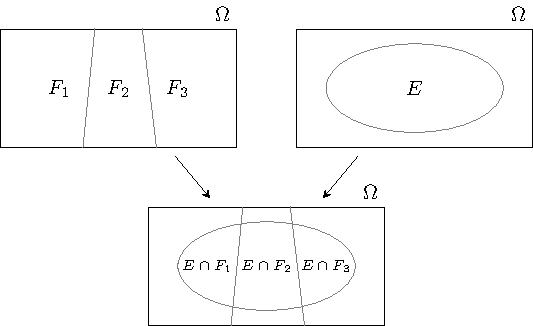
\includegraphics[width=0.8\linewidth]{017_bayes_theorem_files/figure-latex/tikz-prob-tot-1} 

}

\caption{Partizione dello spazio campionario $\Omega$.}\label{fig:tikz-prob-tot}
\end{figure}

\begin{example}
Si considerino tre urne, ciascuna delle quali contiene 100 palline:

\begin{itemize}
\tightlist
\item
  Urna 1: 75 palline rosse e 25 palline blu,
\item
  Urna 2: 60 palline rosse e 40 palline blu,
\item
  Urna 3: 45 palline rosse e 55 palline blu.
\end{itemize}

\noindent
Una pallina viene estratta a caso da un'urna anch'essa scelta a caso.
Qual è la probabilità che la pallina estratta sia di colore rosso?

Sia \(R\) l'evento ``la pallina estratta è rossa'' e sia \(U_i\) l'evento che
corrisponde alla scelta dell'\(i\)-esima urna. Sappiamo che
\[
P(R \mid U_1) = 0.75, \qquad P(R \mid U_2) = 0.60, \qquad P(R \mid U_3) = 0.45.
\]
Gli eventi \(U_1\), \(U_2\) e \(U_3\) costituiscono una partizione dello
spazio campionario in quanto \(U_1\), \(U_2\) e \(U_3\) sono eventi
mutualmente esclusivi ed esaustivi, \(P(U_1 \cup U_2 \cup U_3) = 1.0\). In
base al teorema della probabilità totale, la probabilità di estrarre una
pallina rossa è

\begin{align}
P(R) &= P(R \mid U_1)P(U_1)+P(R \mid U_2)P(U_2)+P(R \mid U_3)P(U_3)\notag\\
&= 0.75 \cdot \frac{1}{3}+0.60 \cdot \frac{1}{3}+0.45 \cdot \frac{1}{3} =0.60.\notag
\end{align}
\end{example}

\begin{example}
Consideriamo un'urna che contiene 5 palline rosse e 2 palline verdi. Due
palline vengono estratte, una dopo l'altra. Vogliamo sapere la
probabilità dell'evento ``la seconda pallina estratta è rossa''.

Lo spazio campionario è \(\Omega = \{RR, RV, VR, VV\}\). Chiamiamo \(R_1\)
l'evento ``la prima pallina estratta è rossa'', \(V_1\) l'evento ``la prima
pallina estratta è verde'', \(R_2\) l'evento ``la seconda pallina estratta è
rossa'' e \(V_2\) l'evento ``la seconda pallina estratta è verde''. Dobbiamo
trovare \(P(R_2)\) e possiamo risolvere il problema usando il teorema
della probabilità
totale~\eqref{eq:prob-total-1b}:

\begin{align}
P(R_2) &= P(R_2 \mid R_1) P(R_1) + P(R_2 \mid V_1)P(V_1)\notag\\
&= \frac{4}{6} \cdot \frac{5}{7} + \frac{5}{6} \cdot \frac{2}{7} = \frac{30}{42} = \frac{5}{7}.\notag
\end{align}

Se la prima estrazione è quella di una pallina rossa, nell'urna restano
4 palline rosse e due verdi, dunque, la probabilità che la seconda
estrazione produca una pallina rossa è uguale a 4/6. La probabilità di
una pallina rossa nella prima estrazione è 5/7. Se la prima estrazione è
quella di una pallina verde, nell'urna restano 5 palline rosse e una
pallina verde, dunque, la probabilità che la seconda estrazione produca
una pallina rossa è uguale a 5/6. La probabilità di una pallina verde
nella prima estrazione è 2/7.
\end{example}

\hypertarget{la-regola-di-bayes}{%
\section{La regola di Bayes}\label{la-regola-di-bayes}}

Il teorema di Bayes rappresenta uno dei fondamenti della teoria della
probabilità e della statistica. Lo presentiamo qui considerando un
caso specifico per poi descriverlo nella sua forma più generale.

Sia \(\{F_1, F_2\}\) una partizione dello spazio campionario \(\Omega\).
Consideriamo un terzo evento \(E \subset \Omega\) con probabilità non
nulla di cui si conoscono le probabilità condizionate rispetto ad \(F_1\)
e a \(F_2\), ovvero \(P(E \mid F_1)\) e \(P(E \mid F_2)\). È chiaro per le
ipotesi fatte che se si verifica \(E\) deve anche essersi verificato
almeno uno degli eventi \(F_1\) e \(F_2\). Supponendo che si sia verificato
l'evento \(E\), ci chiediamo: qual è la probabilità che si sia verificato
\(F_1\) piuttosto che \(F_2\)?

\begin{figure}[h]

{\centering 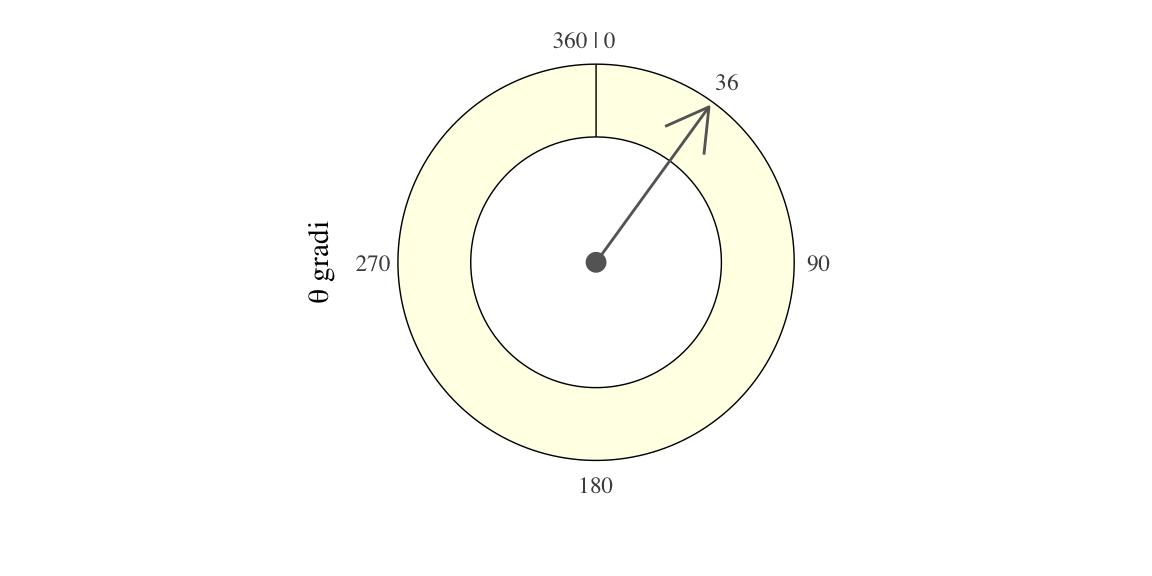
\includegraphics[width=0.45\linewidth]{017_bayes_theorem_files/figure-latex/unnamed-chunk-1-1} 

}

\end{figure}

Per rispondere alla domanda precedente scriviamo:

\begin{align}
P(F_1 \mid E) &= \frac{P(E \cap F_1)}{P(E)}\notag\\ 
              &= \frac{P(E \mid F_1)P(F_1)}{P(E)}.\notag
\end{align}

Sapendo che \(E = (E \cap F_1) \cup (E \cap F_2)\) e che \(F_1\) e \(F_2\) sono eventi disgiunti, ovvero \(F_1 \cap F_2 = \emptyset\), ne segue che possiamo calcolare \(P(E)\) utilizzando il teorema della probabilità totale:

\begin{align}
P(E) &= P(E \cap F_1) + P(E \cap F_2)\notag\\ 
     &= P(E \mid F_1)P(F_1) + P(E \mid F_2)P(F_2).\notag
\end{align}

\noindent
Sostituendo il risultato precedente nella formula della probabilità condizionata \(P(F_1 \mid E)\) otteniamo:

\begin{equation}
P(F_1 \mid E) = \frac{P(E \mid F_1)P(F_1)}{P(E \mid F_1)P(F_1) + P(E \mid F_2)P(F_2)}.
\label{eq:bayes1}
\end{equation}

\noindent
La~\eqref{eq:bayes1} si generalizza facilmente al caso di più di due eventi disgiunti, come indicato di seguito.

\begin{theorem}
\protect\hypertarget{thm:theobayes}{}{\label{thm:theobayes} }Sia \(E\) un evento contenuto in \(F_1 \cup \dots \cup F_k\), dove gli eventi \(F_j, j=1, \dots, k\) sono a due a due incompatibili e necessari. Allora per ognuno dei suddetti eventi \(F_j\) vale la seguente formula:

\begin{equation}
P(F_j \mid E) = \frac{P(E \mid F_j)P(F_j)}{\sum_{j=1}^{k}P(F_j)P(E \mid F_j)}.
\label{eq:bayes2}
\end{equation}
\end{theorem}

\noindent
La~\eqref{eq:bayes2} prende il nome di \emph{Teorema di Bayes} e mostra che la conoscenza del verificarsi dell'evento \(E\) modifica la probabilità che abbiamo attribuito all'evento \(F_j\). Nella \eqref{eq:bayes2} la probabilità condizionata \(P(F_j \mid E)\) prende il nome di probabilità \emph{a posteriori} dell'evento \(F_j\): il termine ``a posteriori'' sta a significare ``dopo che è noto che si è verificato l'evento \(E\)''.
Nel capitolo \ref{chapter-intro-bayes-inference} estenderemo questa discussione mostrando come la \eqref{eq:bayes2} possa essere formulata in un modo più generale, ovvero in modo tale che non faccia riferimento unicamente alla probabilità di eventi, ma bensì anche alle funzioni di densità di probabilità.

\hypertarget{le-probabilita-come-grado-di-fiducia}{%
\subsection{Le probabilità come grado di fiducia}\label{le-probabilita-come-grado-di-fiducia}}

Il teorema di Bayes rende esplicito il motivo per cui la probabilità non può essere pensata come uno stato oggettivo, quanto piuttosto come un'inferenza soggettiva e condizionata. Il denominatore del membro di destra della \eqref{eq:bayes2} è un semplice fattore di normalizzazione. Nel numeratore compaiono invece due quantità: \(P(F_j\)) e \(P(E \mid F_j)\). La probabilità \(P(F_j\)) è la probabilità \emph{probabilità a priori} (\emph{prior}) dell'evento \(F_j\) e rappresenta l'informazione che l'agente bayesiano possiede a proposito dell'evento \(F_j\). Diremo che \(P(F_j)\) codifica il grado di fiducia che l'agente ripone in \(F_j\), sul quale non possiamo porre vincoli di alcun tipo. La probabilità condizionata \(P(E \mid F_j)\) rappresenta invece la verosimiglianza di \(F_j\) e ci dice quant'è plausibile che si verifichi l'evento \(E\) condizionatemente al fatto che si sia verificato \(F_j\).

Nell'interpretazione bayesiana \(P(F_j)\) rappresenta un giudizio personale dell'agente e non esistono criteri esterni che possano determinare se tale giudizio sia coretto o meno. Il teorema di Bayes descrive la regola che l'agente deve seguire per aggiornare il suo grado di fiducia in \(F_j\) alla luce di un ulteriore evento \(E\). Per questo motivo abbiamo chiamato \(P(F_j \mid E)\) probabilità a posteriori: essa rappresenta infatti la nuova probabilità che l'agente assegna ad \(F_j\) affinché rimanga consistente con le nuove informazioni fornitegli da \(E\).

La probabilità a posteriori dipende sia da \(E\), sia dalla conoscenza a priori dell'agente \(P(F_j)\). In questo senso è chiaro come non abbia senso parlare di una probabilità oggettiva: per il teorema di Bayes la probabilità è definita condizionatamente alla probabilità a priori, la quale a sua volta, per definizione, è un'assegnazione soggettiva. Ne segue pertanto che ogni probabilità debba essere una rappresentazione del grado di fiducia (soggettiva) dell'agente.

Se ogni assegnazione probabilistica rappresenta uno stato di conoscenza, è altresì vero che un particolare stato di conoscenza è arbitrario e dunque non deve esserci necessariamente accordo a priori tra diversi agenti. Tuttavia, alla luce di nuove informazioni, la teoria delle probabilità ci fornisce uno strumento che consente l'aggiornamento dello stato di conoscenza in un modo razionale.

\hypertarget{aggiornamento-bayesiano}{%
\subsection{Aggiornamento bayesiano}\label{aggiornamento-bayesiano}}

Il teorema di Bayes consente di modificare una credenza a priori in maniera dinamica, via via che nuove evidenze vengono raccolte, in modo tale da formulare una credenza a posteriori la quale non è mai definitiva, ma può sempre essere aggiornata in base alle nuove evidenze disponibili. Questo processo si chiama \emph{aggiornamento bayesiano}.

\begin{example}
Supponiamo che, per qualche strano errore di produzione, una fabbrica
produca due tipi di monete. Il primo tipo di monete ha la caratteristica
che, quando una moneta viene lanciata, la probabilità di osservare
l'esito ``testa'' è 0.6. Per semplicità, sia \(\theta\) la probabilità di
osservare l'esito ``testa''. Per una moneta del primo tipo, dunque,
\(\theta = 0.6\). Per una moneta del secondo tipo, invece, la probabilità
di produrre l'esito ``testa'' è 0.4. Ovvero, \(\theta = 0.4\).

Noi possediamo una moneta, ma non sappiamo se è del primo tipo o del secondo tipo. Sappiamo solo che il 75\% delle monete sono del primo tipo e il 25\% sono del secondo tipo. Sulla base di questa conoscenza \emph{a priori} -- ovvero sulla base di una conoscenza ottenuta senza avere eseguito
l'esperimento che consiste nel lanciare la moneta una serie di volte per
osservare gli esiti prodotti -- possiamo dire che la probabilità di una
prima ipotesi, secondo la quale \(\theta = 0.6\), è 3 volte più grande
della probabilità di una seconda ipotesi, secondo la quale
\(\theta = 0.4\). Senza avere eseguito alcun esperimento casuale con la
moneta, questo è quello che sappiamo.

Ora immaginiamo di lanciare una moneta due volte e di ottenere il
risultato seguente: \(\{T, C\}\). Quello che ci chiediamo è: sulla base di
questa evidenza, come cambiano le probabilità che associamo alle due
ipotesi? In altre parole, ci chiediamo qual è la probabilità di ciascuna
ipotesi alla luce dei dati che sono stati osservati: \(P(H \mid y)\),
laddove \(y\) sono i dati osservati. Tale probabilità si chiama
probabilità a posteriori. Inoltre, se confrontiamo le due ipotesi, ci
chiediamo quale valore assuma il rapporto \(\frac{P(H_1 \mid y)}{P(H_2 \mid y)}\).
Tale rapporto ci dice quanto è più probabile \(H_1\) rispetto ad \(H_2\), alla luce dei dati osservati.
Infine, ci chiediamo come cambia il rapporto definito sopra, quando osserviamo via via nuovi risultati prodotti dal lancio della moneta.

Definiamo il problema in maniera più chiara.
Conosciamo le probabilità a priori, ovvero \(P(H_1) = 0.75\) e \(P(H_1) = 0.25\).
Quello che vogliamo conoscere sono le probabilità a posteriori \(P(H_1 \mid y)\) e
\(P(H_2 \mid y)\).

Per trovare le probabilità a posteriori applichiamo il teorema di Bayes:
\[
P(H_1 \mid y) = \frac{P(y \mid H_1) P(H_1)}{P(y)} = 
\frac{P(y \mid H_1) P(H_1)}{P(y \mid H_1) P(H_1) + P(y \mid H_2) P(H_2)}
\]
laddove lo sviluppo del denominatore deriva da un'applicazione del teorema della probabilità totale.
Inoltre,
\[
P(H_2 \mid y) = 
\frac{P(y \mid H_2) P(H_2)}{P(y \mid H_1) P(H_1) + P(y \mid H_2) P(H_2)}.
\]
Se consideriamo l'ipotesi \(H_1\) = ``la probabilità di testa è 0.6'', allora
la verosimiglianza dei dati \(\{T, C\}\), ovvero la probabilità di osservare questa specifica sequenza di T e C, è uguale a \(0.6 \times 0.4 = 0.24.\)
Dunque, \(P(y \mid H_1) = 0.24\).

Se invece consideriamo l'ipotesi \(H_2\) = ``la probabilità di testa è 0.4'', allora la verosimiglianza dei dati \(\{T, C\}\) è \(0.4 \times 0.6 = 0.24\), ovvero, \(P(y \mid H_2) = 0.24\).
In base alle due ipotesi \(H_1\) e \(H_2\), dunque, i dati osservati hanno la
medesima plausibilità di essere osservati.
Per semplicità, calcoliamo anche
\[
\begin{aligned}
P(y) &= P(y \mid H_1) P(H_1) + P(y \mid H_2) P(H_2) = 0.24 \cdot 0.75 + 0.24 \cdot 0.25 = 0.24.\notag
\end{aligned}
\]

Le probabilità a posteriori diventano:
\[
\begin{aligned}
P(H_1 \mid y) &= \frac{P(y \mid H_1) P(H_1)}{P(y)} = \frac{0.24 \cdot 0.75}{0.24} = 0.75,\notag
\end{aligned}
\]
\[
\begin{aligned}
P(H_2 \mid y) &= \frac{P(y \mid H_2) P(H_2)}{P(y)} = \frac{0.24 \cdot 0.25}{0.24} = 0.25.\notag
\end{aligned}
\]
Possiamo dunque concludere dicendo che, sulla base dei dati osservati, l'ipotesi \(H_1\) ha una probabilità 3 volte maggiore di essere vera dell'ipotesi \(H_2\).

È tuttavia possibile raccogliere più evidenze e, sulla base di esse, le probabilità a posteriori cambieranno.
Supponiamo di lanciare la moneta una terza volta e di osservare croce.
I nostri dati dunque sono \(\{T, C, C\}\).

Di conseguenza, \(P(y \mid H_1) = 0.6 \cdot 0.4 \cdot 0.4 = 0.096\) e \(P(y \mid H_2) = 0.4 \cdot 0.6 \cdot 0.6 = 0.144\).
Ne segue che le probabilità a posteriori diventano:
\[
\begin{aligned}
P(H_1 \mid y) &= \frac{P(y \mid H_1) P(H_1)}{P(y)} = \frac{0.096 \cdot 0.75}{0.096 \cdot 0.75 + 0.144 \cdot 0.25} = 0.667,\notag
\end{aligned}
\]
\[\begin{aligned}
P(H_2 \mid y) &= \frac{P(y \mid H_2) P(H_2)}{P(y)} = \frac{0.144 \cdot 0.25}{0.096 \cdot 0.75 + 0.144 \cdot 0.25} = 0.333.\notag\end{aligned}\]
In queste circostanze, le evidenze che favoriscono \(H_1\) nei confronti
di \(H_2\) sono solo pari ad un fattore di 2.

Se otteniamo ancora croce in un quarto lancio della moneta, i nostri
dati diventano: \(\{T, C, C, C\}\).
Ripetendo il ragionamento fatto sopra,
\(P(y \mid H_1) = 0.6 \cdot 0.4 \cdot 0.4 \cdot 0.4 = 0.0384\) e
\(P(y \mid H_2) = 0.4 \cdot 0.6 \cdot 0.6 \cdot 0.6 = 0.0864\).

Dunque
\[
\begin{aligned}
P(H_1 \mid y) &= \frac{0.0384 \cdot 0.75}{0.0384 \cdot 0.75 + 0.0864 \cdot 0.25} = 0.571,\notag
\end{aligned}
\]
\[
\begin{aligned}
P(H_2 \mid y) &= \frac{0.0864 \cdot 0.25}{0.0384 \cdot 0.75 + 0.0864 \cdot 0.25} = 0.429.\notag
\end{aligned}
\]
e le evidenze a favore di \(H_1\) si riducono a 1.33. Se si ottenesse un
altro esito croce in un sesto lancio della moneta, l'ipotesi \(H2\)
diventerebbe più probabile dell'ipotesi \(H_1\).

In conclusione, questo esercizio ci fa capire come sia possibile aggiornare le nostre credenze sulla base delle evidenze disponibili, ovvero come sia possibile passare da un grado di conoscenza del mondo a priori a una conoscenza a posteriori.
Se prima di lanciare la moneta ritenevamo che l'ipotesi \(H_1\) fosse tre volte più plausibile dell'ipotesi \(H_2\), dopo avere osservato uno specifico campione di dati siamo giunti alla conclusione opposta.
Il processo di aggiornamento bayesiano, dunque, ci fornisce un metodo per modificare il livello di fiducia in una data ipotesi, alla luce di nuove informazioni.
\end{example}

\hypertarget{considerazioni-conclusive}{%
\section*{Considerazioni conclusive}\label{considerazioni-conclusive}}
\addcontentsline{toc}{section}{Considerazioni conclusive}

Il teorema di Bayes costituisce il fondamento dell'approccio più moderno
della statistica, quello appunto detto bayesiano. Chi usa il teorema di
Bayes non è, solo per questo motivo, ``bayesiano'': ci vuole ben altro. Ci
vuole un modo diverso per intendere il significato della probabilità e
un modo diverso per intendere gli obiettivi dell'inferenza statistica. In anni recenti, una gran parte della comunità scientifica ha riconosciuto all'approccio bayesiano il merito di consentire lo sviluppo di modelli anche molto complessi (intrattabili in base all'approccio frequentista) senza richiedere, d'altra parte, conoscenze matematiche troppo avanzate all'utente. Per questa ragione l'approccio bayesiano sta prendendo sempre più piede, anche in psicologia.

\hypertarget{appendix-appendix}{%
\appendix}



% Bibliography
%%%%%%%%%%%%%%%%%%%%%%%%%%%%%%%%%%%%%%%%%%%%%%%%%%%%%%%%%%

\backmatter
\SmallMargins

\printbibliography
\onecolumn


% Tables (of tables, of figures)
%%%%%%%%%%%%%%%%%%%%%%%%%%%%%%%%%%%%%%%%%%%%%%%%%%%%%%%%%%


\cleardoublepage
\LargeMargins
\listoffigures


% After-body (LaTeX code inclusion)
%%%%%%%%%%%%%%%%%%%%%%%%%%%%%%%%%%%%%%%%%%%%%%%%%%%%%%%%%%




% Back cover
%%%%%%%%%%%%%%%%%%%%%%%%%%%%%%%%%%%%%%%%%%%%%%%%%%%%%%%%%%%

% Even page, small margins, no running head, no page number.
\evenpage
\SmallMargins
\thispagestyle{empty}

\begin{normalsize}

\begin{description}

\selectlanguage{italian}
\item[Abstract]
This document contains the material of the lessons of Psicometria B000286 (2021/2022) aimed at students of the first year of the Degree Course in Psychological Sciences and Techniques of the University of Florence, Italy.
\item[Keywords]
Data science, Bayesian statistics.
~\\

\end{description}

\end{normalsize}


\end{document}
